\documentclass[12pt]{report}

\usepackage[utf8]{inputenc}
\usepackage{t1enc}
\usepackage[magyar]{babel}
\usepackage{amsmath}
\usepackage{url}
\usepackage{graphicx}

\graphicspath{ {./latex_images} }

\newcommand*{\xdash}[1][3em]{\rule[0.5ex]{#1}{0.55pt}}
\newcommand*{\ydash}[1][0.9em]{\rule{0.55pt}{#1}}


\title{Structure from Motion from Two Views}
\date{}

\begin{document}
    \maketitle

    \chapter{Algoritmus}
    A Structure from motion (SfM) folyamat segítségével 3D rekonstrukciót hajthatunk végre egy képpár segítségével.

    \begin{enumerate}
        \item Két kép közötti ritka ponthalmazok megfeleltetése (pontmegfeleltetés): az első kép sarokpontjainak azonosítása a \textit{detectMinEigenFeatures} függvénnyel, majd azok követése a második képre a \textit{vision.PointTracker} segítségével.
        \item Az esszenciális mátrix becslése \textit{estimateEssentialMatrix} használatával.
        \item Kamera elmozdulásának kiszámítása \textit{estrelpose} függvénnyel.
        \item Két kép közötti sűrű ponthalmazok megfeleltetése (pontmegfeleltetés): több pont kinyeréséhez újra kell detektálni a pontokat a \textit{detectMinEigenFeatures} függvény segítségével a \textit{'MinQuality'} opciót használva. Ezt követi a sűrű ponthalmaz követése a második képre a \textit{vision.PointTracker} használatával.
        \item Az illeszkedő pontok 3D helyzeteinek meghatározása a \textit{triangulate} segítségével (háromszögelés).
    \end{enumerate}    

    \chapter{Kód magyarázata}
        \section{Képpár betöltése}
            \begin{enumerate}
                \item \textit{fullfile(string1, string2, ...)} = az argumentumként kapott stringekből összeállít egy elérési útvonalat, pl.:\\\\
                    \texttt{path = fullfile('myfolder', 'mysubfolder')\\path = 'myfolder\textbackslash mysubfolder\textbackslash '}\\\\
                    \textit{toolboxdir(toolbox)} = visszaadja az argumentumként kapott toolbox abszolút elérési útvonalát.
                \item \textit{imageDatastore(path)} = létrehoz egy ImageDatastore objektumot a kapott elérési útvonallal meghatározott képekből. Az ImageDatastore objektum segítségével egy mappában található összes képet össze lehet gyűjteni egy változóba (de alapból nem lesz az összes kép egyszerre betöltve).
                \item \textit{readimage(datastore, n)} = betölti az n. képet a megadott datastore-ból.
                \item \textit{figure} = létrehoz egy új, üres ábra ablakot.
                \item \textit{imshowpair(image1, image2, 'montage')} = a meghatározott két képet egymás mellé helyezi a legutolsó ábrán.
                \item \textit{title('string')} = hozzáad egy címet a legutolsó ábrához.
            \end{enumerate}

        \section{A Camera Calibrator alkalmazás segítségével előre kiszámolt kamera paraméterek betöltése.}
            \begin{enumerate}
                    \item \textit{load(file\_name.mat)} = betölti egy korábban elmentett workspace adatait a jelenlegi workspace-be. A workspace egy ideiglenes tároló amely a MATLAB elindítása óta létrehozott változókat tárolja. Alapértelmezetten a MATLAB ablak jobb oldalán látható. A workspace-t el lehet menteni, így a benne tárolt változókat később vissza lehet tölteni a MATLAB-ba.
            \end{enumerate}

        \section{Lencse által okozott torzítás eltávolítása.}
            \begin{enumerate}
                \item \textit{undistortImage(image, intrinsics)} = a második argumentumként megadott kamera paramétereket felhasználva eltűnteti a kamera lencséje által okozott torzítást a megadott képről.\\
                      A kamera kalibrációja során kapott kamera paramétereket és a torzítási együtthatókat felhasználva kiszámítjuk a bemeneti kép minden pixelének eredeti pozícióját. Az egyes pixelek pozícióját az alábbi torzítások módosítják:
                        \begin{itemize}
                            \item \textbf{Radiális torzítás} = kiváltó oka, hogy a lencse szélén áthaladó fény jobban törik, mint a lencse közepén környezetében áthaladó fény. Ez kiszámolható:\\
                                \[x_r = x(1 + k_1r^2 + k_2r^4)\]
                                \[y_r = y(1 + k_1r^2 + k_2r^4)\]
                                (Ahol $x_r, y_r$ = radiális torzulásmentes koordináták; $x, y$ = torzított koordináták; $k_1, k_2$ = radiális torzítási együtthatók; $r^2 = x^2 + y^2$)
                            \item \textbf{Tangenciális fordítás} = előfordul, ha a kameraszenzor és a lencse nem állnak tökéletesen párhuzamosan. Ez kiszámolható:\\
                                \[x_t = 2p_1xy + p_2(r^2+2x^2)\]
                                \[y_t = 2p_2xy + p_1(r^2 + 2y^2)\]
                                (Ahol $x_t, y_t$ = tangenciális torzulásmentes koordináták; $x, y$ = torzított koordináták; $p_1, p_2$ = tangenciális torzítási együtthatók; $r^2 = x^2 + y^2$)\\\\
                                A végső együttható értékének kiszámítása:
                                \[x_f = x_r + x_t\]
                                \[y_f = y_r + y_t\]
                    Az egyes pixelek korrigált helyének kiszámítása nem egész számú értékeket is előállít. Mivel a nem egész szám nem lehet pixel koordináta, ezért bilineáris interpolációt is végre kell hajtani. A bilineáris interpoláció során, a legközelebbi négy szomszédot felhasználva először lineáris interpolációt hajtunk végre az egyik irányba (pl. az x tengely mentén), majd pedig a másik irányba (az y tengely mentén):
                        \[out_P = I_1(1 - \Delta X)(1 - \Delta Y) + I_2 (\Delta X)(1 - \Delta Y) + I_3(1 - \Delta X)(\Delta Y) + I_4(\Delta X)(\Delta Y)\]
                        (Ahol $I_1, I_2, I_3, I_4$ = a szomszédos négy koordináta intenzitása az eredeti, torzított képen; $\Delta X, \Delta Y$ = a nem egész értékű koordinátákkal rendelkező vizsgált pixel és a vizsgált pixelhez legközelebb eső, egész értékű koordinátákkal rendelkező szomszédai közötti távolság; $out_P$ = végeredményként kapott pixel intenzitás)\\\\
                    A szomszédos pixelek efféle súlyzott átlagolásával, az interpoláció eredményeképp egy pixel intenzitás értéket kapunk, amely a legközelebbi egész érték koordinátával rendelkező pixel intenzitása lesz.\\
                    Az előállított, torzítatlan képen néhány pixel (leginkább a kép szélein) nem rendelkezik megfelelő pixel párral az eredeti, torzított képről (ezek azok a területek, ahol az eredeti képből nincs információ). Ezek a pixelek alapértelmezetten 0 értéket kapnak (feketék lesznek). 
                        \end{itemize}
                \end{enumerate}

            \section{Pontmegfeleltetés a képek között.}
                \begin{enumerate}
                    \item \textit{detectSURFFeatures(grayImage, "MetricThreshold", value)} = A Speeded Up Robust Features (SURF) a SIFT algoritmus továbbfejlesztésének is tekinthető. \\
                    \begin{enumerate}
                        \item \textbf{Integrál kép létrehozása} = A számítások gyorsítása érdekében létrehozzuk a bementi kép integrál képét. Az integrál kép egy olyan reprezentáció, amely minden pontban a bal felső saroktól addig a pontig lévő intenzitásértékek összegét tárolja: \\
                        \[I_{\sum}(x, y) = \sum_{i=0}^{x} \sum_{j=0}^{y} I(i, j)\]
                        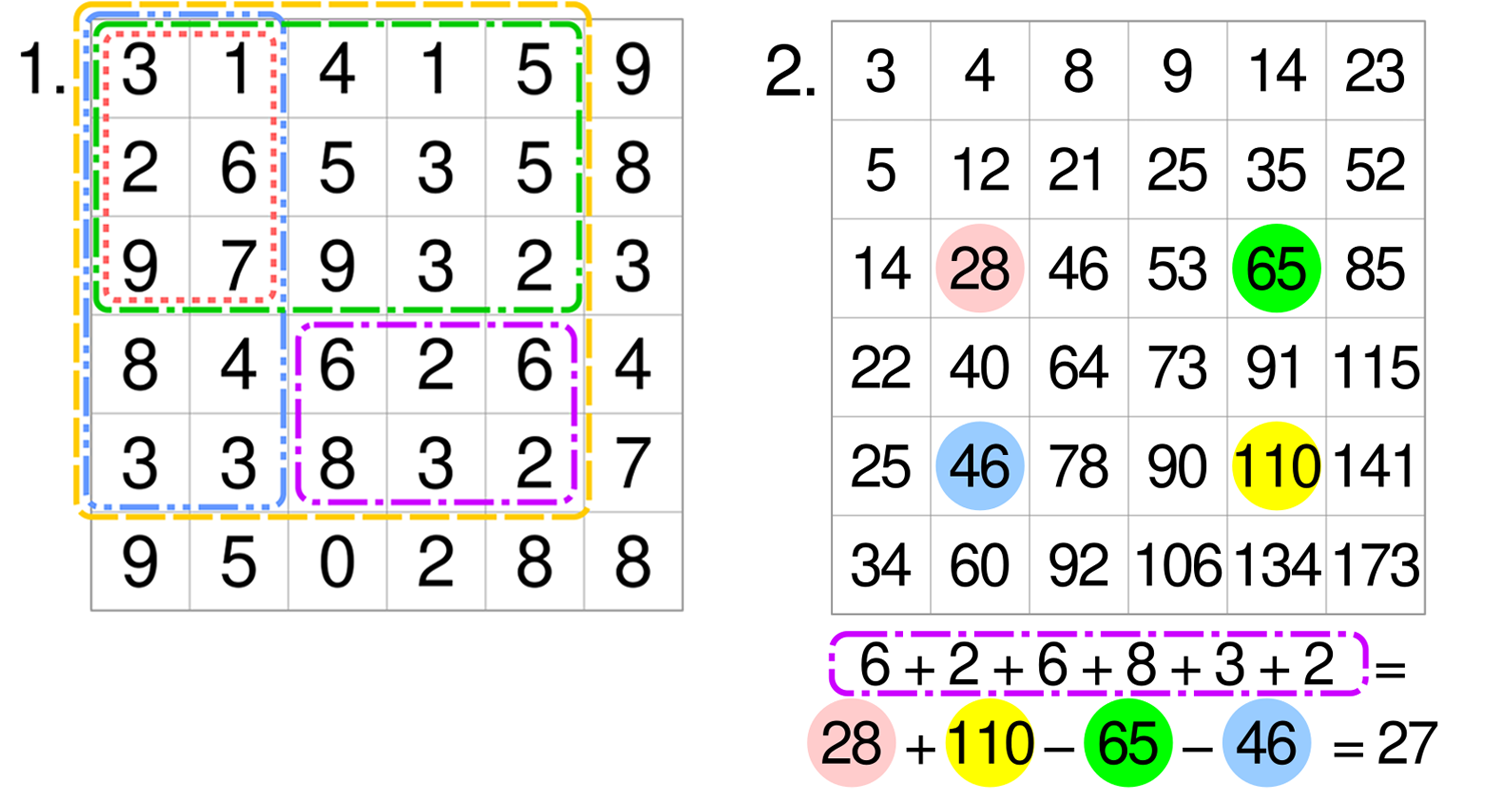
\includegraphics[scale=0.2]{integral_image.png}\\
                        Az integál kép felhasználásával gyorsan ki lehet a pixelértékek összegét az adott képen vagy annak egy meghatározott részterületén. Pl.:\\
                        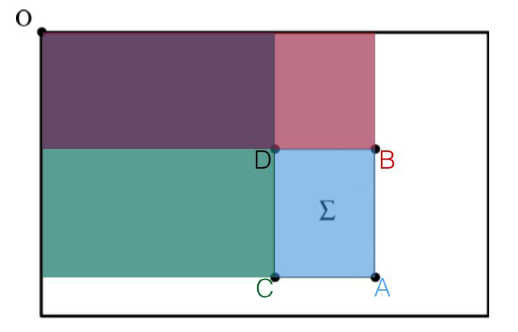
\includegraphics[scale=0.4]{Summed_area_table.png}\\
                        \[\sum = A - B - C + D\]
                        A kulcspontok megkeresésére a teljesítmény optimalizálása érdekében SURF algoritmus a Hess-mátrixot használja. A kulcspontok pozícióját és a skáláját is a Hess mátrix determinánsának közelítésével számoljuk. A Hess determináns approximálásához a SURF a további teljesítménynövelés eléréséhez ún. dobozszűrőt (\textit{box filter}) használ. A doboz szűrő egy olyan szűrő, amely minden, egy előre meghatározott ablakon belüli képpontok értékét a környező pixelek átlagaival helyettesíti. Ennél a folyamatnál nagyon hasznos az integrált kép, ugyanis bármely képpontra meg tudjuk mondani az őt megelőző pixelek értékeinek összegét (gyorsítva a számolást). Ezen lépés után a Hess mátrix determinánsának approximáltja:
                        \[det(H_{approx}) = D_{xx}D_{yy} - (wD_{xy})^2\]
                        ahol:
                        \begin{itemize}
                            \item \textit{$D_{xx}$}, \textit{$D_{yy}$}, \textit{$D_{xy}$} = másodrendű képpont deriváltak horizontális, vertikális és keresztirányban
                            \item \textit{w} = dobozszűrő ablakára vonatkozó súly (általban 0.9)
                        \end{itemize}
                    \end{enumerate}
                        

                    \item \textit{imshow(image, InitialMagnification = value)} = a meghatározott kép megjelenítése \textit{value}\%-os megnagyításban.
                    \item \textit{hold on} = a következőkben végrehajtott grafikus (pl.: grafikonok kirajzolása, stb.) parancsokat a legutolsó, aktuális ábrára fogja rárajzolni.
                    \item \textit{plot} = létrehoz kétdimenziós grafikont.
                    \item \textit{selectStrongest(featurePoints, N)} = visszaadja az \textit{N} legerősebb (talán ez az intenzitások különbségének nagyságát jelenti) jellemzőpontot (nálunk sarokpontok lesznek) a megadott \textit{featurePoints} változóból.
                    \item \textit{tracker = vision.PointTracker(MaxBidirectionalError=value1, NumPyramidLevels=value2)} = létrehoz egy Kanade-Lucas-Tomasi (KLT) algoritmus szerint működő pontkövető objektumot.\\
                    A KLT algoritmus kifejezetten jól működik olyan objektumok követésére, amely nem változtat alakot, valamint egyedi és részletes textúrával rendelkezik. A KLT algoritmus a Lucas-Kanade (LK) optikai áramlás becslés algoritmuson alapul. Az optikai áramlás az objetumok egy látszólagos/vizuális elmozdulása (nem feltétlenül egyezik meg a valós elmozdulással). Általános feltételezése, hogy egy objektum megfigyelt pixeleinek intenzitása elmozdulástól függetlenül állandó:
                    \[I(x,y,t) = I(x + u,y + v,t + 1)\]
                    Ahol:
                    \begin{itemize}
                        \item \textit{I(x,y,t)} = \textit{(x,y)} pozíción lévő pixel intenzitása \textit{t} időben
                        \item \textit{u} = elmozdulás az x tengelyen
                        \item \textit{v} = elmozdulás az y tengelyen
                    \end{itemize}

                    Ebből kifejezhető az optikai áramlás egyenlete Taylor sort alkalmazva:
                    \[I(x + u,y + v,t + 1) \approx I(x,y,t) + I_xu + I_yv + I_t\]
                    \[I(x + u,y + v,t + 1) - I(x,y,t) = I_xu + I_yv + I_t\]
                    \[0 \approx I_xu + I_yv + I_t\]
                    Ahol:
                    \begin{itemize}
                        \item \textit{$I_xu$} = az intenzitás változása az x tengelyen.
                        \item \textit{$I_yv$} = az intenzitás változása az y tengelyen.
                        \item \textit{$I_t$} = az intentizás idő szerinti változása.
                    \end{itemize}
                    Tehát, ha az \textit{u} és \textit{v} elmozdulások helyesen vannak meghatározva, akkor az intenzitások különbsége megközelítőleg 0. Azonban \textit{u} és \textit{v} ismeretlenek és meghatározásukat nehezíti a \textbf{nyílás/rekesz/apertúra probléma (aperture problem)}, azaz amikor a tényleges mozgást egy kicsi rekeszen keresztül figyelve próbáljuk meghatározni. Egy objektum tényleges elmozdulásának kiszámítása nehéz, ha csak egy kis területet látunk belőle a résen keresztül.\\
                    A Lucas-Kanade algoritmus feltételezi, hogy az optikai áramlás (\textit{u} és \textit{v}) konstans és a képen textúrázott tárgyak láthatók. A megfigyelt pixel kezdeti intenzitása \textit{a}, valamint a rés mögött látható tárgy elmozdítása után észlelt pixel intenzitása \textit{b}. Ezek különbsége \textit{(b - a)}, azaz az időbeli intenzitáskülönbség \textit{$I_t(x,y)$}. A \textit{(x,y)} pozíción megfigyelt pixel intenzitásváltozás \textit{$I_x(x,y)$} az x tengelyen, valamint \textit{$I_y(x,y)$} az y tengelyen. Az x tengelyen történő \textit{u} mértékű és az y tengelyen történő \textit{v} mértékű elmozdulás esetén a pixel intenzitása:
                    \[I_x(x,y)u + I_y(x,y)v = -I_t(x,y)\]
                    Nem tudom miért negatív az $I_t$ :(\\\\
                    Az algoritmus helyes működéséhez nem elegendő egyetlen pixelt nézni, így ezt ki kell terjeszteni egy pixelszomszédságra. Egy 3x3 szomszédság esetén az egyenlet:
                    \[I_x(x + \Delta x, y + \Delta y)u + I_y(x + \Delta x, y + \Delta y)v = -I_t(x + \Delta x, y + \Delta y)\] ahol $\Delta x$ = -1,0,1 (a három szomszédos pixel az x tengelyen), $\Delta y$ = -1,0,1 (a három szomszédos pixel az y tengelyen)
                    Tömör formában a képlet:
                    \[S\begin{bmatrix} u \\ v \end{bmatrix} = \overset{\rightarrow}{t}\]
                    Ahol:
                    \begin{itemize}
                        \item \textit{S} = 9x2 mátrix amely tartalmazza: $[I_x(x + \Delta x, y + \Delta y),  I_y(x + \Delta x, y + \Delta y]$.
                        \item \textit{$\overset{\rightarrow}{t}$} = vektor amely tartalmazza: $-I_t(x + \Delta x, y + \Delta y)$.
                    \end{itemize}
                    Ezen két ismeretlenes egyenlet megoldása a legkisebb négyzetek módszerével történik, amihez megszorozzuk az egyenletet $S^{T}$ (én sem értem miért):
                    \[S^{T}S\begin{bmatrix}u \\ v\end{bmatrix} = S^{T}\overset{\rightarrow}{t}\]
                    Ebből $\begin{bmatrix}u \\ v\end{bmatrix}$ kifejezve:
                    \[\begin{bmatrix}u \\ v\end{bmatrix} = (S^{T}S)^{-1}S^{T}\overset{\rightarrow}{t}\]
                    Röviden (ha jól fogtam fel) a Lucas-Kanade optikai áramlás becslés algoritmusa a képkockák közötti mozgást próbálja nyomon követni. Ehhez két képkockán kiválaszt egy pixelszomszédságot és azok térbeli elmozdulását elemzi. Ezután kiszámolja a pixelértékek intenzitásváltozását, amelyből próbálja kiszámolni az objektum tényleges elmozdulását. Gyorsan mozgó vagy nem ritkásan textúrázott objektumok esetén nem megbízható.\\
                    A tényleges pontmegfeleltetést a Kanade-Lucas-Tomasi (KLT) algoritmus végzi, amelyből a MATLAB vision.PointTracker függvény a pyramid KLT továbbfejlesztett verziót használja. Először minden kiválasztott jellemzőponthoz egy kis ablakot/apertúrát illeszt. A következő lépésben létrehoz egy kép piramist: a kiinduló képből több szintet hoz létre, ahol az alsó szinten található a teljes (eredeti) felbontású kép, a piramis teteje felé haladva a vizsgált kép egyre kisebb felbontású verziója fog szerepelni. Ezután kiszámolja a kiválasztott pixelek elmozdulás vektorait a piramis legfelső szintjétől kezdve, az előbb tárgyalt Lucas-Kanade optikai áramlás becslés algoritmusát felhasználva. A becsült mozgásokat használva finomítja a jellemzőpontok pozícióit a következő alacsonyabban elhelyezkedő, magasabb felbontású piramisszinten. Ezt addig folytatja, amíg el nem éri a legalsó szintet. A piramisos módszer előnye, hogy az alacsonyabb felbontású képeken végzett kezdeti nyomkövetés javítja a teljes nyomkövetési pontosságot és akár nagyobb távolságok követését is lehetővé teszi.\\
                    A \textit{vision.PointTracker} függvényhívásnál használt két argumentum:
                    \begin{itemize}
                        \item \textit{MaxBidirectionalError} = a funkció lényege, hogy az épp vizsgált pontot az első képről követi a második képre, majd ugyanazon pontot követi visszafelé a második képről az első képre. Ezután kiszámolja a vizsgált pont eredeti és a visszakövetés utáni, új pozíciója közötti különbséget (az első képen). Ha ez az érték nagyobb, mint az függvénynek átadott \textit{MaxBidirectionalError} érték, akkor az adott pont érvénytelen. Hatékony módszer a nem megbízhatóan követhető pontok kiküszöbölésére. Az ajánlott érték 0 és 3 pixel között van.
                        \item \textit{NumPyramidLevels} = a képpiramis szintjeinek számát határozza meg. A nagyobb érték lehetővé teszi a nagyobb elmozdulások követését, viszont lassabb futási időt eredményez. Az ajánlott érték 1 és 4 között van.
                    \end{itemize}
                    \item \textit{imagePoints1 = imagePoints1.Location} = a sarokpont objektumok pozícióinak kiolvasása.
                    \item \textit{initialize(pointTracker, points, image1)} = inicializálja az első argumentumként kapott pontkövető objektumot, inicializálja a második argumentumként kapott követendő pontokat, valamint beállítja az utolsó argumentumként kapott képet a kezdeti képkockának.
                    \item \textit{[returnValue1, returnValue2] = step(tracker, image2)} = a \textit{step} függvény indítja el az első argumentumként kapott pontkövető objektumot. A függvény második argumentum a második képkocka, amelyen el kell végeznie a pontkövetést az objektumnak. Az első visszatérési érték a korábban meghatározott jellemzőpontok koordinátái a második képkockán. A második visszatérési érték egy logikai indexvektor, amely azt jelzi, hogy mely pontokat sikerült nyomon követni. A megbízhatóan követhető pontok \textit{true}, míg ellenkező esetben \textit{false} értéket kapnak.
                    \item \textit{matchedPoints = imagePoints(validIdx, :)} = a megbízhatóan követhető pontok lementése. Az \textit{imagePoints} egy mátrix, melynek sorai tartalmazzák a jellemzőpontokat, két oszlopai pedig a jellemzőpontok x és y koordinátáit. A \textit{imagePoints(validIdx, :)} rész egy mátrix címzés, amely visszaadja mátrix azon sorait ahol \textit{validIdx} = \textit{1} vagy \textit{true}, valamint a mátrix összes oszlopát (: jelentése összes index).
                    \item \textit{showMatchedFeatures(image1, image2, matchedPoints1, matchedPoints2)} = a pontmegfeleltetés eredményének kirajzolása. A két agumentumként kapott kép színkódolást kap, valamint a másik két, argumentumként kapott jellemzőpontok is kirajzolódnak és egy vonallal lesznek összekötve a hozzájuk tartozó párjukkal.
                    \item \textit{[returnValue1, returnValue2] = estimateEssentialMatrix(matchedPoints1, matchedPoints2, intrinsics)} = az esszenciális mátrix becslése egy képpár megfeleltetett pontjaiból.\\
                    Az esszenciális mátrix két kamera közötti mozgást kapcsolja össze, megfeleltetett pontpárok közötti geometriai kapcsolatok leírásával. Tehát a különböző szögből készült képekhez használt kamerák relatív helyzetét és orientációját segít meghatározni, \textbf{ha} ismertek a kamera paraméterek (amiket a kamera kalibrációjakor kapunk meg).\\
                    Az esszenciális mátrix egy 3x3 szerkezetű, homogén, 2-es rangú mátrix, amely az alábbi alapján írja le a két képkocka közötti kapcsolatot (\textit{koplanaritási egyenlet}):
                    \[x_1^TEx_2 = 0\]
                    Az $x_1$ egy adott pont homogén koordinátája az első képen, míg az $x_2$ ugyanazon pont homogén koordinátája a második képen (mindkét esetben a kamera koordináta rendszerében, nem pedig pixel koordináta rendszerben):
                    \[x_1 = \begin{bmatrix}x_1\\y_1\\1\end{bmatrix}, x_2 = \begin{bmatrix}x_2\\y_2\\1\end{bmatrix}\]
                    A két képpont kapcsolatát leíró egyenlőség szerint, ha a két képpont ugyanazon pontot írják le, akkor az esszenciális mátrix ($E$) segítségével kifejezhető a köztük lévő kapcsolat. A képlet szétbontva:\\
                    \[\begin{bmatrix}x_1&y_1&1\end{bmatrix}\begin{bmatrix}E_{11}&E_{12}&E_{13}\\E_{21}&E_{22}&E_{23}\\E_{31}&E_{32}&E_{33}\end{bmatrix}\begin{bmatrix}x_2\\y_2\\1\end{bmatrix} = 0\]
                        \hspace{3cm} $\overset{\uparrow}{ismert}$ \hspace{1cm} $\overset{\uparrow}{ismeretlen}$ \hspace{0.1cm} $\overset{\uparrow}{ismert}$\\
                    Ha elvégezzük az ismert elemek szorzatát, majd szétválasztjuk az ismeretlen az ismert részektől:
                    \[A\begin{bmatrix}E_{11}\\\vdots\\E_{33}\end{bmatrix} = 0\]
                    Ezt szinguláris érték felbontással végezhetjük el, megkapva az esszenciális mátrixot. Ezt a módszert 8 pont algoritmusnak hívják, amely minimum 8 pontpárt és normalizált koordinátákat követel meg.
                    Az esszenciális mátrix két alapvető elemből áll:
                    \[E = [t]_xR\]
                    Ahol:
                    \begin{itemize}
                        \item \textit{R} = egy ortogonális 3x3-as rotációs mátrix amely a kamerák közötti forgást írja le: $R = \begin{bmatrix}r_{11}&r_{12}&r_{13}\\r_{21}&r_{22}&r_{23}\\r_{31}&r_{32}&r_{33}\end{bmatrix}$
                        \item \textit{[$t_x$]} = a \textit{t} egy transzlációs vektor, amely a kamera két pozíciójának közötti eltolást írja le: $t = \begin{bmatrix}t_x\\t_y\\t_z\end{bmatrix}$. \textit{[$t_x$]} = a transzlációs vektor ferde mátrixa (\textit{skew-symmetric matrix}, én sem tudom mi az), amely biztosítja, hogy a vektorok közötti keresztszorzat mátrixművelettel leírható legyen: $[t]_x = \begin{bmatrix}0&-t_z&t_y\\t_z&0&-t_x\\-t_y&t_x&0\end{bmatrix}$\\
                    \end{itemize}
                    Ez a rész valószínűleg erősen hiányos, de nem teljesen értem, hogy hogyan történik az esszenciális mátrix becslése.\\
                    A második visszatérési érték, az \textit{epipolarInliers} megadja, hogy a megfeleltetett pontok mennyire esnek közel az epipoláris síkhoz. (Ha jól értelmeztem) az epipoláris sík magyarázata:\\
                    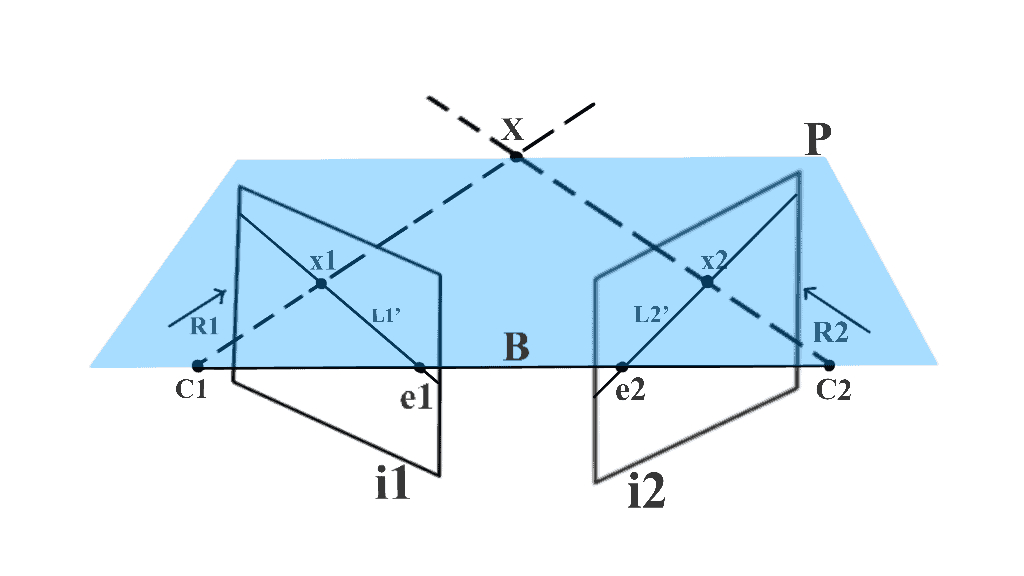
\includegraphics[scale=0.4]{epipolar_line.jpg}
                    Az X pontról készítünk egy-egy képet két különböző szemszögből (a kamera középpontja az első pozícióban $C_1$, míg a második pozícióban lévő kamera középpontja $C_2$). Az első képen az X pont $x_1$ pontban, míg a második képen $x_2$ pontban lett megörökítve. Ha húzunk egy vonalat a $C_1$ középpontból a képen szereplő $x_1$ ponton túl, a vonal át fog haladni a lefényképezett X ponton, azaz az első képen $x_1$ pont a $C_1$ kameraközéppont és a lefényképezett X pont közé húzott vonalon helyezkedik el (ez a vonal az $R_1$). Ha ez a vonal látható lenne, akkor a második képen látható részlete lenne a második képhez tartozó epipoláris vonal ($L_2$). Ahogy az első képen az $x_1$ az $R_1$ vonalon helyezkedik el, úgy a második képen az $x_2$ pontnak is az $L_2$ epipoláris vonalon kell elhelyezkednie.\\
                    A MATLAB \textit{estimateEssentialMatrix} függvény egy \textit{MSAC} elnevezésű algoritmust használ, hogy eldöntse mely pontok outlierek (az epipoláris síktól messze találhatóak) és melyek az inlierek (az epipoláris síkhoz közel találhatóak). Mivel a megfeleltetett képpontoknak az epipoláris síkon kellene elhelyezkedniük, az outlierek rosszul lettek párosítva a pontmegfeleltetés során, így ezeket kiszűrjük.
                    \item \textit{inlierPoints = matchedPoints(epipolarInliers, :)} = lementsük az epipoláris vonalhoz közel eső (tehát a valószínűleg helyesen párosított) pontokat.
                    \item \textit{estrelpose(essentialMatrix,intrinsics,inlierPoints1,inlierPoints2)} = kiszámítja a második kamera relatív pozícióját az elsőhöz képest az esszenciális mátrixból kinyert rotációs mátrix és transzlációs vektor alapján. Nem találtam meg, hogy pontosan hogyan teszi ezt :(
                    \item \textit{camProjection = cameraProjection(intrinsics,tform)} = a visszatérési értéke egy kamera vetítési mátrix. Homogén koordinátával rendelkező, 3D pontok képre való vetítésére szolgál az argumentumként kapott \textit{tform} transzformáció szerint, valamint a kamera belső paramétereit is figyelembe véve.\\
                    A vetítési mátrix egy 3x4 szerkezetű mátrix, amely leírja a kamera valóvilágbéli, 3D pontok leképezését 2D pontokra a képsíkra/elkészült képre:
                    \[x = PX\]
                    Ahol:
                    \begin{itemize}
                        \item \textit{x} = 2D képpont = $\begin{bmatrix}X\\Y\\Z\end{bmatrix}$
                            \item \textit{P} = kamera mátrix = $K\begin{bmatrix}R|t\end{bmatrix}$, ahol \textit{K} = a kamera belső paraméterei, \textit{R} = rotációs mátrix, \textit{t} = transzlációs mátrix.
                            \item \textit{X} = 3D pont a valóvilágban = $\begin{bmatrix}X\\Y\\Z\\1\end{bmatrix}$
                    \end{itemize}
                    Az alkalmazott merev transzformáció (\textit{rigidtform3d}) egy olyan transzformáció, amelybe beletartozik a forgatás és eltolás, de nem változtatja meg az objektum méretét és formáját. Ha nem adunk meg semmilyen argumentumot, akkor a \textit{rigidtform3d} egy identitás transzformációt hajt végre, amely semmilyen módon nem változtatja meg az objektumot a leképezés során (forgatást és eltolást is beleértve). Mivel az első kamera a referenciapontunk (tehát az első kamera az origón található), ezért csak egységtranszformációt hajtunk végre.
                    A kamera mátrix kiszámítása a meghatározott transzformációval:
                    \[P = K\begin{bmatrix}rigidtform3d.R|rigidtform3d.t\end{bmatrix}\]
                   
                    A mátrix tartalmazza a képre vetített 3D pontokat homogén koordinátákban.\\
                    A második kamera esetében az első kamera szerinti relatív elhelyezkedést és orientációt (\textit{relPose}) átadjuk a \textit{pose2extr} függvénynek, amely visszaadja a kamera külső paramétereit (extrinsic mátrix). A kamera külső paraméterei azt mutatják meg, hogyan kell a kamera koordináta-rendszeréből a világ koordináta-rendszerébe végrehajtani a transzformációt. Ez azt jelenti, hogy ha van egy pont a kamera koordináta-rendszerében, akkor a \textit{pose2extr} által visszaadott extrinsic mátrix segítségével átalakíthatjuk ezt a pontot a világ koordináta-rendszerébe. Innentől fogva a \textit{cameraProjection} függvény a belső és külső paramétereket felhasználva leírja a második kamerához tartozó kamera vetítési mátrixot. (Nem tudom mennyire helyes ez a bekezdés).
                    \item \textit{triangulate(matchedPoints1, matchedPoints2, camProjection1, camProjection2)} = Az argumentumként kapott pontpárok és kamera vetítési mátrixok segítségével háromszögelést végez. Visszatérési értéke a megfeleltetett pontpárok világkoordináta-rendszerbeli koordinátái.\\
                    Az előző pontokban említettük, hogy a kamera mátrix megadja a 3D pont képsíkra történő 2D leírását:
                    \[x = PX\]
                Mivel ismert az \textit{x} és a \textit{P} elméletben ebből az X könnyen meghatározható:\\
                    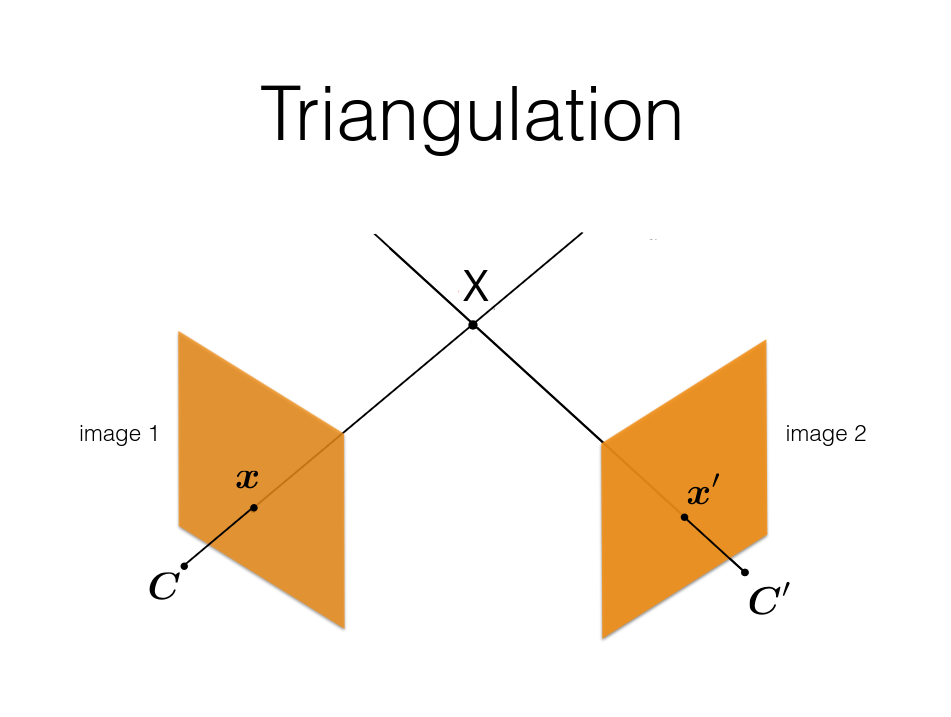
\includegraphics[scale=0.4]{triangulation.png}
                    \begin{itemize}
                        \item \textit{C} = az első kamera középpontja.
                        \item \textit{C'} = a második kamera középpontja.
                        \item \textit{x} = az első kamera \textit{X} objektumról készített leképezése az első képsíkra.
                        \item \textit{x'} = a második kamera \textit{X} objektumról készített leképezése a második képsíkra.
                        \item \textit{X} = az eredeti 3D objektum.
                    \end{itemize}
                    Elméletben tehát ha húzunk egy vetítősugarat az első kamera középpontjából kezdve, át az \textit{x} ponton, valamint húzunk még egy vetítősugarat a második kamera középpontjától kezdve, át az \textit{x'} ponton, a két egyenes metszéspontja meg kell határoznia \textit{X} pontot. A probléma, hogy ehhez tökéletes mérések kellenek, a valóságban viszont a különböző zajok és mérési pontatlanságok miatt  a két vetítősugár nem fogja metszeni egymást. Ennek következtében a valóságban csak közelítő eredményt keresünk. A háromszögelés lináris megoldása: \\
                    Szétbontjuk az alábbi egyenletet:\\
                    \[x = PX\]
                    \[\begin{bmatrix}x\\y\\z\end{bmatrix} = 
                        \begin{bmatrix}
                        p_{11} & p_{12} & p_{13} & p_{14} \\
                        p_{21} & p_{22} & p_{23} & p_{24} \\
                        p_{31} & p_{32} & p_{33} & p_{34}
                        \end{bmatrix}
                        \begin{bmatrix}X\\Y\\Z\\1\end{bmatrix}\]
                        Vesszük a P mátrix sorait és transzponáljuk:
                        \[\begin{bmatrix}x\\y\\z\end{bmatrix} = 
                        \begin{bmatrix}
                        \xdash & p_{1}^T & \xdash \\
                        \xdash & p_{2}^T & \xdash \\
                        \xdash & p_{3}^T & \xdash
                        \end{bmatrix}
                        \begin{bmatrix}\ydash\\X\\\ydash\end{bmatrix}\]
                        A mátrix egyes sorait szorozzuk az \textit{X} vektorral:
                        \[\begin{bmatrix}x\\y\\z\end{bmatrix} =
                        \begin{bmatrix}
                        p_{1}^TX\\
                        p_{2}^TX\\
                        p_{3}^TX
                        \end{bmatrix}\]
                        Vesszük az egyenlőség két oldalának keresztszorzatát:
                        \[\begin{bmatrix}x\\y\\z\end{bmatrix} \times \begin{bmatrix}
                        p_{1}^TX\\
                        p_{2}^TX\\
                        p_{3}^TX
                        \end{bmatrix} = 0\]
                        (\textit{Két párhuzamos vektor keresztszorzata 0. Keresztszorzatot az alábbi minta szerint végzünk:
                        \[a \times b = \begin{bmatrix} 
                            a_2 b_3 - a_3 b_2 \\ 
                            a_3 b_1 - a_1 b_3 \\ 
                            a_1 b_2 - a_2 b_1 
                            \end{bmatrix}
                        \]})
                        \[\begin{bmatrix}
                        yp_3^TX - p_2^TX \\
                        p_1^TX - xp_3^TX \\
                        xp_2^TX - yp_1^TX
                        \end{bmatrix} = 0\]
                        A harmadik sor az első két sor kombinációja (az első sor \textit{x}-szer, és a második sor \textit{y}-szor), az a sor jelenleg nem jelentős, így azt elhagyjuk.\\
                        Az eddigi eljárást megcsináljuk mindkét kamera esetében:
                        \[\begin{bmatrix}
                        yp_3^{T}X - p_2^{T}X \\
                        p_1^{T}X - xp_3^{T}X \\
                        \end{bmatrix} = 0, 
                        \begin{bmatrix}
                        y^{'}p_3^{'T}X - p_2^{'T}X \\
                        p_1^{'T} - x'p_3^{'T}X \\
                        \end{bmatrix} = 0\]
                        A két mátrixot összeillesztjük és kiemeljük az \textit{X}-et:
                        \[\begin{bmatrix}
                        yp_3^{T} - p_2^{T} \\
                        p_1^{T} - xp_3^{T} \\
                        y^{'}p_3^{'T} - p_2^{'T} \\
                        p_1^{'T} - x'p_3^{'T}
                        \end{bmatrix}X = 0\]
                        A mátrixot egy \textit{A}-val jelöljük:
                        \[AX = 0\]
                        Ez az egyenlőség pedig szinguláris értékek felbontásával (SVD) oldható, megkapva a pont közelítő, 3D koordinátáját.
                        \item \textit{numPixels = size(var, dim1) * size(var, dim2)} = a \textit{size} függvény visszatérési értéke a \textit{var} változó mérete a meghatározott \textit{dim1} dimenzióban (\textit{1} = sorok száma, \textit{2} = oszlopok száma). A mi példánkban az egyenlettel lekérjük a kép magasságát és szélességét, ezek szorzatával pedig kiszámítsuk a kép pixeleinek számát.
                        \item \textit{allColors = reshape(I1, [numPixels, 3])} = a megadott képet átalakítjuk egy tömbbé, amelynek minden sora a kép egy pixele, az oszlopai pedig az adott sorban található pixel RGB értékét adja meg.
                        \item \textit{colorIdx = sub2ind([size(I1, 1), size(I1, 2)], round(matchedPoints1(:,2)),round(matchedPoints1(:, 1)))} = A megfeleltetett pontok indexeinek kiolvasása. Az indexeket subscript (sor és oszlop indexek) típusból lineáris indexszé (az index egy darab szám, amely az oszlopok mentén haladva a legelső elemtől kezdődik) alakítjuk.
                        \item \textit{color = allColors(colorIdx, :)} = kiolvassuk a megfeleltetett pontok színeit az indexvektor segítségével.
                        \item \textit{pointCloud(xyzPoints, colors)} = meghatározott színekkel létrehozza a pontfelhő objektumot.
                        \item \textit{figure\\
                                      plotCamera(Size=cameraSize, Color="r", Label="1", Opacity=0);\\
                                      hold on\\
                                      grid on\\
                                      plotCamera(AbsolutePose=relPose, Size=cameraSize,Color="b", Label="2", Opacity=0)} = kirajzoljuk az első kamerát az origóba piros színnel, majd pedig a második kamerát kék színnel az első kamera pozíciójától a kiszámolt relatív pozícióba.
                \end{enumerate}

    \chapter{Forrás}
        \begin{itemize}
            \item \url{https://www.mathworks.com/help/vision/ug/structure-from-motion-from-two-}\\\url{views.html}
            \item \url{https://www.mathworks.com/help/vision/ref/undistortimage.html?s_tid=doc_ta}
            \item \url{https://www.mathworks.com/help/visionhdl/ug/image-undistort.html}
            \item \url{https://e-learning.ujs.sk/pluginfile.php/23441/mod_resource/content/1/01-ProjektivKamera.pdf}
            \item \url{https://www.mathworks.com/help/vision/ref/detectmineigenfeatures.html}
            \item \url{https://aishack.in/tutorials/features/}
            \item \url{https://aishack.in/tutorials/harris-corner-detector/}
            \item \url{https://aishack.in/tutorials/shitomasi-corner-detector/}
            \item \url{https://docs.opencv.org/3.4/dc/d0d/tutorial_py_features_harris.html}
            \item \url{https://www.mathworks.com/help/vision/ref/vision.pointtracker-system-object.html}
            \item \url{https://lorenzopeppoloni.com/lkttracker/}
            \item \url{https://www.baeldung.com/cs/optical-flow-lucas-kanade-method}
            \item \url{https://www.inf.u-szeged.hu/~kato/teaching/IpariKepfeldolgozas/08-Motion.pdf}
            \item \url{http://www.inf.fu-berlin.de/inst/ag-ki/rojas_home/documents/tutorials/Lucas-Kanade2.pdf}
            \item \url{https://link.springer.com/chapter/10.1007/978-3-319-29451-3_29}
            \item \url{https://www.mathworks.com/help/matlab/ref/step.html}
            \item \url{https://www.mathworks.com/help/vision/ref/showmatchedfeatures.html}
            \item \url{https://www.baeldung.com/cs/fundamental-matrix-vs-essential-matrix}
            \item \url{https://e-learning.ujs.sk/pluginfile.php/23450/mod_resource/content/1/05-SztereoKamera.pdf}
            \item \url{https://learnopencv.com/introduction-to-epipolar-geometry-and-stereo-vision/}
            \item \url{https://www.mathworks.com/help/vision/ref/estrelpose.html}
            \item \url{https://www.mathworks.com/help/vision/ref/cameraprojection.html}
            \item \url{https://ksimek.github.io/2012/08/14/decompose/}
            \item \url{https://www.cs.cmu.edu/~16385/s17/Slides/11.1_Camera_matrix.pdf}
            \item \url{https://www.mathworks.com/help/images/ref/rigidtform3d.html}
            \item \url{https://www.storyofmathematics.com/rigid-transformation/}
            \item \url{https://staff.fnwi.uva.nl/r.vandenboomgaard/ComputerVision/LectureNotes/CV/StereoVision/triangulation.html}
            \item \url{https://e-learning.ujs.sk/pluginfile.php/23450/mod_resource/content/1/05-SztereoKamera.pdf}
        \textbf{SURF}
            \item \url{https://en.wikipedia.org/wiki/Summed-area_table}
            \item \url{https://www.cs.umd.edu/class/spring2020/cmsc426-0201/files/14_SURF.pdf}
            \item \url{https://link.springer.com/chapter/10.1007/11744023_32}
            \item \url{https://docs.opencv.org/3.4/df/dd2/tutorial_py_surf_intro.html}
            \item \url{https://medium.com/@deepanshut041/introduction-to-surf-speeded-up-robust-features-c7396d6e7c4e}
        \end{itemize}
\end{document}
